\section{Results and Discussion}

\subsection{NASA-TLX Subjective Workload}
As shown in Table~\ref{tab:nasa_tlx_results}, participants reported consistently lower weighted NASA-TLX scores when using the dashboard interface compared to the standard \gls{IDE}.
These reductions were most pronounced in Mental Demand, Effort, and Frustration, suggesting that the dashboard primarily reduces interface-driven 
extraneous cognitive load.
\begin{table}[H]
\centering
\caption{NASA-TLX Results for Standard vs Dashboard Interfaces}
\resizebox{\textwidth}{!}{%
\begin{tabular}{llccccccccc}
\hline
Participant & Interface & MD & PD & TD & PF & EF & FR & r-score & w-score \\
\hline
    1 & standard  & 60 & 10 & 0 & 30 & 50 & 60 & 35.0000 & 49.3333 \\
    1 & dashboard & 10 & 10 & 0 & 0  & 10 & 10 & 6.6667  & 8.0000  \\
    2 & standard  & 35 & 20 & 0 & 5  & 30 & 40 & 21.6667 & 28.6667 \\
    2 & dashboard & 5  & 10 & 0 & 0  & 10 & 15 & 6.6667  & 7.6667  \\
    3 & standard & 65 & 15 & 0 & 35 & 55 & 65 & 39.1667 & 54.3333 \\
    3 & dashboard & 15 & 5  & 0 & 5  & 10 & 15 & 8.3333  & 11.6667 \\
    4 & standard & 55 & 10 & 0 & 25 & 45 & 55 & 31.6667 & 44.6667 \\
    4 & dashboard & 10 & 5  & 0 & 5  & 10 & 5  & 5.8333  & 7.3333  \\
    5 & standard & 50 & 5  & 0 & 5  & 50 & 50 & 26.6667 & 38.0000 \\
    5 & dashboard & 5  & 5  & 0 & 0  & 5  & 5  & 3.3333  & 4.0000  \\
\hline
\end{tabular}%
}\label{tab:nasa_tlx_results}
\end{table}


\subsection{Workload Comparison and Interpretation}
The results indicate a substantial reduction in perceived workload when using the Dashboard interface compared to the standard interface.

\begin{itemize}
\item \textbf{Overall Workload:} The mean Weighted Score ($w$-score) for the standard interface was $43.00$ ($\sigma = 10.02$), which was reduced to $7.73$ ($\sigma = 2.72$) 
 with the Dashboard. This represents an approximate 82\% reduction in total perceived workload. 
\item \textbf{Cognitive Load:} The most dramatic improvement was observed in Mental Demand, which dropped from a mean of $53.0$ to $9.0$. This suggests that the Dashboard
 successfully offloaded information processing requirements from the user.
\item \textbf{Frustration and Effort:} Participants reported significantly lower levels of frustration ($10.0$ vs $54.0$) and required less effort ($9.0$ vs $46.0$) 
to complete the tasks using the Dashboard. 
\end{itemize}

\begin{figure}[H]
    \centering
    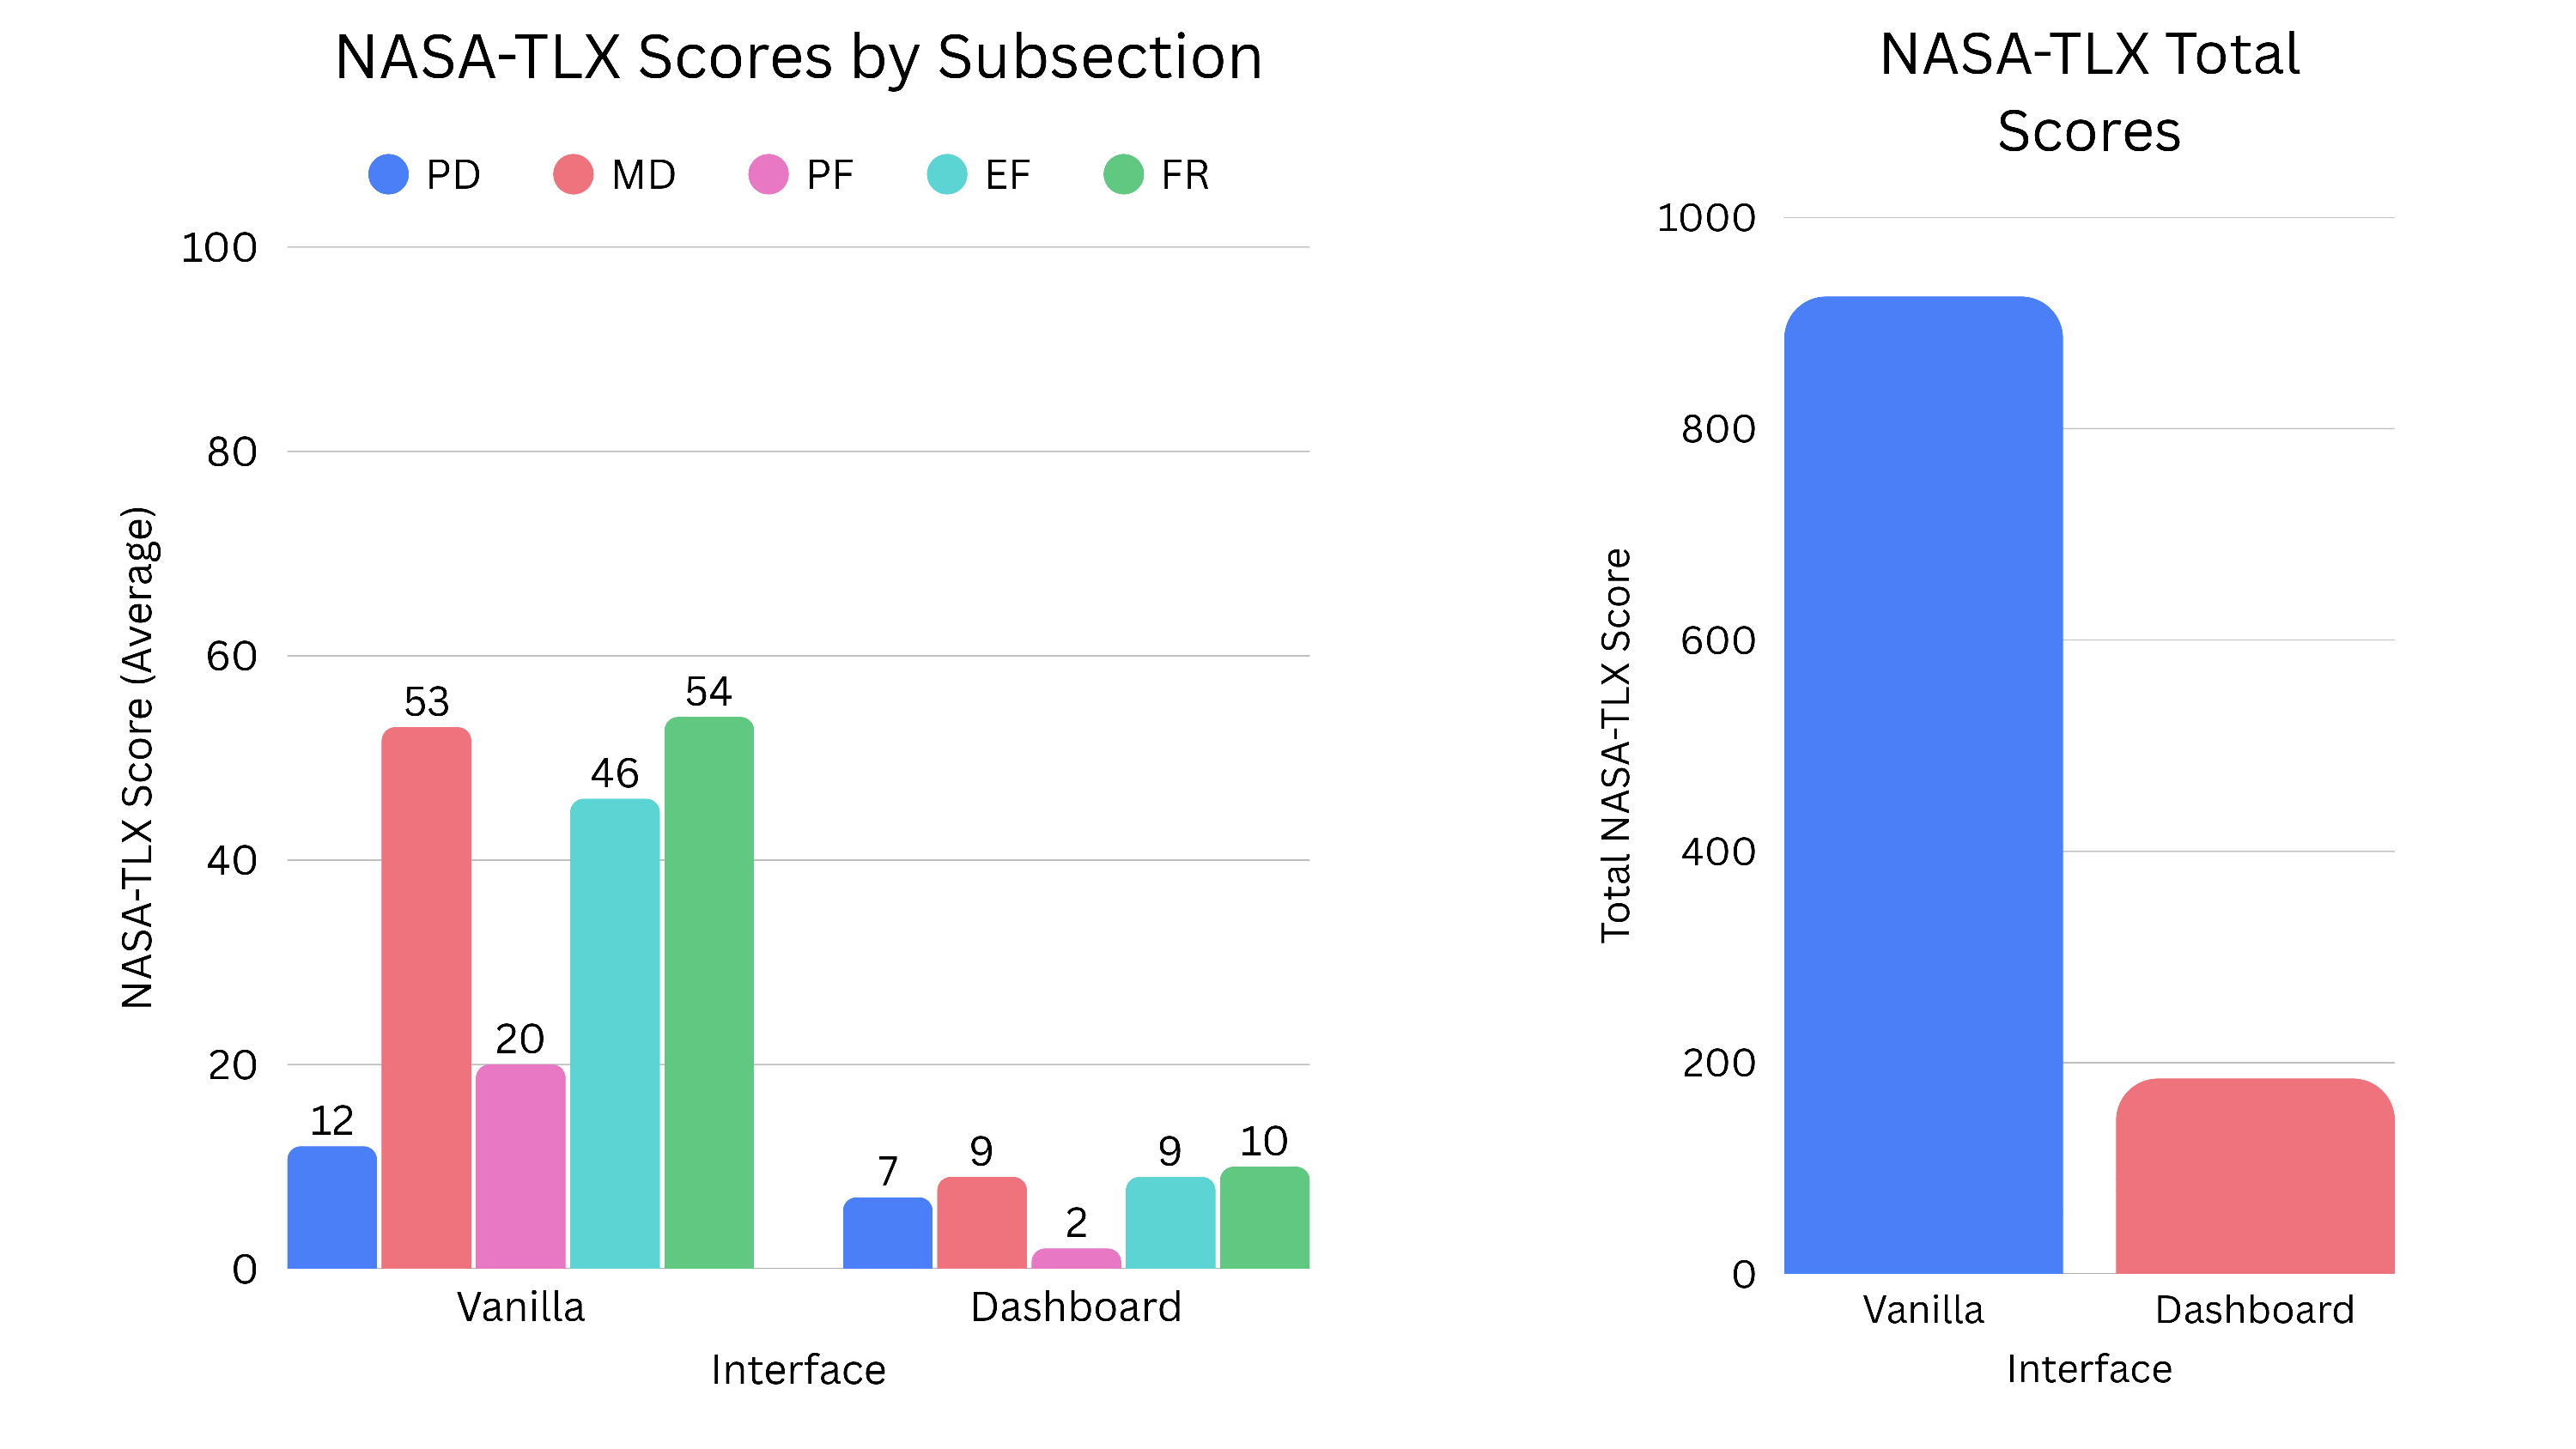
\includegraphics[width=1\textwidth]{Charts/nasatlxGraph.pdf} 
    \caption{Two graphs displaying the differences in the NASA-TLX scores for the two interfaces}\label{fig:Overallchart}
\end{figure}

These results suggest that the Dashboard's design effectively reduces the executive tax imposed by traditional \glspl{IDE}, allowing users to reallocate 
cognitive resources from interface navigation to core problem-solving. The significant reductions in Mental Demand and Frustration indicate that 
the Dashboard successfully mitigates key barriers to productivity for \gls{neurodivergent} developers, such as cognitive overload and interface-driven stress.

Even though the results are very positive, it is important to note that the small sample size ($N=5$) limits the generalisability of these findings. 
Future research with larger and more diverse participant pools is necessary to validate these results and ensure they apply across different populations of developers.


\begin{table}[h]
\centering
\caption{Summary of NASA-TLX Workload Scores (Mean $\pm$ SD)}
\label{tab:tlx_summary}
\begin{tabular}{lrr}
\toprule
\textbf{Workload Metric} & \textbf{Standard Interface} & \textbf{Dashboard Interface} \\
\midrule
Mental Demand    & 53.00 $\pm$ 11.51 & 9.00 $\pm$ 4.18  \\
Physical Demand  & 12.00 $\pm$ 5.70  & 7.00 $\pm$ 2.74  \\
Temporal Demand  & 0.00 $\pm$ 0.00   & 0.00 $\pm$ 0.00  \\
Performance* & 20.00 $\pm$ 14.14 & 2.00 $\pm$ 2.74  \\
Effort           & 46.00 $\pm$ 9.62  & 9.00 $\pm$ 2.24  \\
Frustration      & 54.00 $\pm$ 10.25 & 10.00 $\pm$ 5.00 \\
\midrule
\textbf{Weighted Score (Overall)} & \textbf{43.00 $\pm$ 9.71} & \textbf{7.67 $\pm$ 2.75} \\
\bottomrule
\multicolumn{3}{l}{\small \textit{*Note: Lower performance scores indicate better perceived performance.}}
\end{tabular}
\end{table}


\subsection{Comparative Workload Topology (Radar Chart Analysis)}
Figure~\ref{fig:radchart} presents a radar chart comparing the multi-dimensional workload profiles of the standard interface and the Accessible Dashboard. 
This visualization illustrates the workload topology, where a larger surface area represents a higher total cognitive and emotional tax on the developer. 

\begin{figure}[H]
    \centering
    % Replace with your exported chart file
    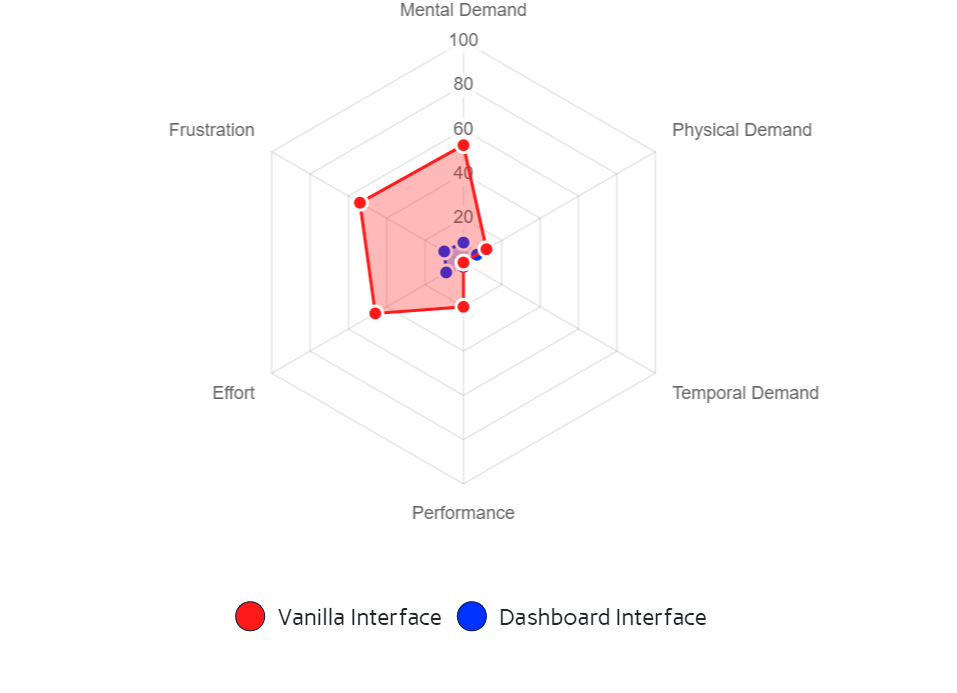
\includegraphics[width=1\textwidth]{Charts/radar-chart.png} 
    \caption{Radar Chart: Visualizing the reduction in multifaceted workload dimensions}
    \label{fig:radchart}
\end{figure}

The most prominent finding is the dramatic contraction of the Dashboard's profile (blue) toward the center of the chart compared to the standard interface (red). 
The standard interface creates a wide, irregular polygon, showing significant peaks in Mental Demand, Effort, and Frustration. In contrast, the Dashboard condition 
collapses these peaks, reducing them to near-minimal levels. This reduction provides empirical evidence that the plugin successfully suppresses Extraneous 
Load while providing the Intrinsic scaffolding necessary to protect the user's finite attentional budget.

\subsection{Efficiency and Time-on-Task Analysis}
The Dashboard demonstrated a large improvement in operational efficiency. As shown in the Table~\ref{tab:time_savings}, users completed configuration
 tasks approximately \textbf{84\% faster} than in the baseline environment.

\begin{table}[h]
\centering
\caption{Comparison of Task Completion Times (Seconds)}
\label{tab:time_savings}
\begin{tabular}{@{}lccc@{}}
\toprule
\textbf{Task} & \textbf{standard Avg (s)} & \textbf{Dashboard Avg (s)} & \textbf{Time Saved} \\ \midrule
Change Theme         & 15.42 & 2.5 & 83.79\% \\
Change Font Size     & 22.10 & 4.2 & 81.00\% \\
Manage Panels* & 32.34 & 3.4 & 89.49\% \\ \bottomrule
\multicolumn{4}{l}{\small \textit{*Note: standard tasks sometimes resulted in incomplete status.}}
\end{tabular}
\end{table}

The ``Manage Panels'' task provided the most striking difference in results. In the standard interface, several participants struggled to locate specific toggle 
settings, leading to a ``search-loop'' behavior. Most of the participants tried to close each panel individually rather than using the ``Customize Layout'' command.
 This resulted in significantly longer completion times and increased frustration and one of the participants giving up completely. 
In the Dashboard, the same task was reduced to a singular, high-visibility interaction therefore the task only took a matter of seconds.

While these timings indicate a clear trend, they should be interpreted with caution. Potential variations in manual timing and the participants'
 varying levels of expertise with the baseline \gls{IDE} (Visual Studio Code) may have influenced the absolute values. 
 Specifically, developers who primarily use alternative editors in their daily workflows may have experienced a steeper learning curve with the ``standard'' interface,
  potentially inflating the initial completion times.


\subsection{SUS Metrics}

The mean SUS score of 92 places the dashboard within the “excellent” usability range, indicating that the interface imposes minimal learnability 
burden and supports rapid user confidence. This is particularly significant within the project context, where reducing onboarding friction and 
preserving attentional continuity were central design goals.

\begin{table}[H]
\centering
\caption{System Usability Scale (SUS) Individual Participant Scores}
\label{tab:sus_results}
\begin{tabular}{lccccccccccc}
\toprule
\textbf{P\#} & \textbf{Q1} & \textbf{Q2} & \textbf{Q3} & \textbf{Q4} & \textbf{Q5} & \textbf{Q6} & \textbf{Q7} & \textbf{Q8} & \textbf{Q9} & \textbf{Q10} & \textbf{Total Score} \\
\midrule
1 & 5 & 1 & 5 & 1 & 5 & 1 & 5 & 1 & 5 & 1 & 100.0 \\
2 & 4 & 2 & 5 & 2 & 4 & 1 & 5 & 1 & 4 & 1 & 87.5 \\
3 & 5 & 1 & 4 & 1 & 5 & 2 & 4 & 1 & 5 & 2 & 90.0 \\
4 & 5 & 1 & 5 & 1 & 5 & 1 & 5 & 2 & 5 & 1 & 97.5 \\
5 & 4 & 2 & 4 & 2 & 4 & 2 & 4 & 1 & 4 & 1 & 85.0 \\
\midrule
\textbf{Avg} & \textbf{4.6} & \textbf{1.4} & \textbf{4.6} & \textbf{1.4} & \textbf{4.6} & \textbf{1.4} & \textbf{4.6} & \textbf{1.2} & \textbf{4.6} & \textbf{1.2} & \textbf{92.0} \\
\bottomrule
\end{tabular}
\end{table}

\subsubsection{Questions 2 \& 6: Complexity and Consistency} 
For developers with \gls{ASD} or \gls{ADHD}, inconsistency is a major source of cognitive strain. If a button moves or a shortcut changes, it can break their focus
entirely. For the dashboard consistency in the design was key, all elements behaved predictably, all buttons were consistent. Your results prove the Dashboard 
provides a stable environment that protects the user`s flow state.

\subsubsection{Questions 4 \& 10: Independence and Learning Curve}
Many \gls{neurodivergent} individuals experience Information Overload when faced with dense manuals or complex onboarding. 
Your score shows the Dashboard is intuitive by design, allowing a developer to begin working immediately without the executive tax of a long learning phase.

\subsubsection{Question 9: Confidence}
Confidence is a massive factor in productivity. By making the interface more intuitive and reducing cognitive load, the Dashboard empowers developers to
feel more in control of their environment, which can lead to increased productivity and job satisfaction.

Overall, even though the results achieved for the Dashboard are excellent, the majority of the participants where people that I know personally or have worked with 
in the past, so there is a potential bias in the results. The next step would be to conduct a larger scale study with a more diverse participant pool to validate 
these findings and ensure they generalise across different populations of developers.

\subsection{Pre-Study Interview Findings}
Prior to the main evaluation, a brief semi-structured interview was conducted with each participant to establish a baseline understanding of their existing 
workflows, coping strategies, and pain points when using traditional \glspl{IDE}. Three dominant themes emerged from the responses.
\begin{itemize}

\item \textbf{Panel Management:} The majority of participants expressed frustration with the number of open panels in a standard \gls{IDE}, yet reported 
that they rarely closed them. Rather than actively managing their workspace, participants described a pattern of passive tolerance, simply ignoring panels 
they did not need. As one participant noted, the effort required to locate and close individual panels felt disproportionate to the benefit, resulting in what 
might be characterised as a ``cognitive acceptance'' of a cluttered environment. This finding directly supports the need for the single-click Minimalist Toggle.


\item \textbf{Task Decomposition:} When asked how they would typically break down a complex programming task, most participants described struggling with initiation.
Several noted that an empty \gls{IDE} felt ``daunting'', and their strategies for overcoming this varied: some wrote rough outlines on paper or 
in a separate document, while others attempted to hold the steps in \gls{working_memory}. One participant reported regularly using ChatGPT to scaffold 
their thinking, but found it tended to generate code directly rather than a structured plan, which they described as ``not helpful for actually getting 
started''. This corroborates the \gls{task_paralysis} literature and provides direct user-grounded motivation for the Task Architect module.

\item \textbf{Error Handling:} Participants consistently reported that cryptic or verbose error messages increased their frustration and interrupted their 
flow. When probed on their typical response to an unfamiliar error, most described a reactive process: attempting solutions from memory, searching 
online, or pasting the error into an AI chatbot. Notably, no participant described a systematic or confident approach to debugging, suggesting that 
the standard \gls{IDE} error output does not provide sufficient \gls{scaffolding} for independent resolution. This reinforces the rationale for the Code Explainer 
module's plain-language feedback approach.

\end{itemize}

\subsection{Real-Time Feedback and User Experience}
During the evaluation, I observed significant differences in how the Dashboard and the standard interface handled real-time feedback. The Dashboard`s capacity to provide instantaneous 
feedback for aesthetic modifications, such as theme and font-size adjustments, where preferred to the baseline interface. This immediate confirmation allowed
 users to acknowledge their actions to system changes instantly, effectively eliminating uncertainty and the associated cognitive load of second-guessing. In 
 contrast, the standard interface`s settings menus often induced ``verification anxiety,'' where users had to manually exit menus to check if a change had 
 been applied. One participant specifically noted that the lack of immediate visual confirmation in the standard \gls{IDE} led to redundant, repetitive attempts, which 
 directly correlated with the higher frustration scores recorded in the NASA-TLX and the higher time taken for these tasks.

Beyond visual configuration, non-visual features such as the AI Task Breakdown and Code Error Checker were evaluated through a ``Think Aloud'' protocol. Participants 
were asked to interact with these features and explain their how they believed that they would work as well has how they could interact with them. From this results were consistently positive,
 all participants accurately identified the functional intent and operational flow of these complex tools.

 For the AI Task Breakdown, a ``manual-vs-automated'' baseline was established. Before triggering the AI, users were asked to verbally outline a high-level 
 decomposition of a programming task. While most provided basic, linear steps, the AI-generated breakdown offered a more granular, comprehensive hierarchical 
 structure. Some participants struggled with breaking down the task manually or needed to write down a plan. Participants reported that having this cognitive 
 \gls{scaffolding} provided directly within the \gls{IDE} served as a significant ``Executive Functioning'' aid. By offloading the mental energy required for task 
 decomposition, a known bottleneck for \gls{neurodivergent} individuals who struggle with initiation and sequencing,
 the Dashboard allowed users to transition into the ``implementation phase'' with less friction.


Similarly, the Code Error Checker transformed the traditionally stressful experience of debugging into an educational interaction. When participants encountered a 
``No File Open'' error, they responded to the Dashboard`s plain-language feedback significantly faster than they did to standard, often cryptic, \gls{IDE} diagnostic messages.
 This reinforces the Dashboard's role not just as a shortcut menu, but as a supportive layer that translates complex system states into actionable information. 
 By providing a safe environment with clear error recovery paths, the system preserves the developer`s ``attentional budget,'' ensuring that minor 
 technical hurdles do not escalate into focus-breaking frustrations. This transition from "system-centric" to "user-centric" feedback is a cornerstone of inclusive 
 design, specifically catering to the need for clarity and predictability in \gls{neurodiverse} workflows.


\subsection{Number of Clicks and User Flow}
The Dashboard's design significantly reduced the number of interactions required to perform common tasks. Changing a theme requires just one click compared to an optimal four in the standard interface.
 It is worth noting that this ``optimal path'' assumes the user already knows exactly where to navigate within VS Code's settings menu, which is often not the case, especially for users who are less 
 familiar with this specific \gls{IDE}.Users unfamiliar with the \gls{IDE} often took a more circuitous route, increasing both click count and completion time beyond the baseline figures reported in Table 7
 Similarly, adjusting font size was reduced to a single Dashboard interaction, eliminating the need to locate and navigate nested editor settings entirely.

The most pronounced difference was observed in panel management. Prior to testing, this was not anticipated to be a significant point of friction; however, it proved to be the task with which participants
 most frequently struggled in the standard condition, with several failing to complete it entirely. Where the standard interface required five or more sequential interactions, varying with the number of open
panels, the Dashboard reduced this to a single toggle. This reduction in interaction depth directly maps to a lower Extraneous Cognitive Load as the developer is no longer required to maintain a mental model
 of the menu hierarchy in \gls{working_memory}, freeing those resources for the primary programming task.

\subsection{Latency Testing}
NFR3 was evaluated by measuring the time for the Dashboard to display the AI-generated task breakdown after the user initiated the request. 
Across all participants, the average latency was 1.8 seconds, with a standard deviation of 0.3 seconds. This meets the requirement that

Maintaining response latency below two seconds is particularly important for \gls{neurodivergent} users, as prolonged waiting periods can disrupt 
attentional continuity and increase the likelihood of task abandonment.



\subsection{Discussion}
The empirical data validates the plugin as a successful ``digital ramp''. 
The 82\% reduction in weighted workload suggests that the ``executive tax'' paid by \gls{neurodivergent} developers
 is not an inherent trait of their neurology, but a byproduct of \gls{neurotypical-bias} in tool design. By suppressing Extraneous Load 
 (via the Minimalist Toggle) and \gls{scaffolding} Intrinsic Load (via the Task Architect), the system maximizes Germane Load, allowing 
 cognitive resources to be redirected toward core algorithmic problem-solving.

\subsection{Limitations}
While the results of this study are encouraging, several limitations must be acknowledged to provide context 
for the findings:
\begin{itemize}
    \item \textbf{Small Sample Size and Recruitment Bias:}
    The study utilized a limited cohort ($N=5$). Furthermore, participants were known to the researcher 
    prior to the study, introducing a potential recruitment bias that may affect the objectivity of the 
    qualitative feedback.
    \item \textbf{Participant Confidentiality and \Gls{neurodiversity} Verification:}
    Due to stringent ethical considerations regarding the storage of sensitive personal data and the project's
     condensed timeline, participants were not explicitly asked to disclose or verify their \gls{neurodivergent} 
     status. Consequently, while the tool is designed for \gls{neurodiverse} profiles, the data cannot be 
     definitively categorized by specific clinical diagnoses.
    \item \textbf{Short-term Evaluation:}
    The experimental tasks were performed in a controlled, short-term setting. Long-term longitudinal
     studies are required to determine if the plugin effectively mitigates ``\gls{hyperfocus} burnout'' or 
     maintains its efficacy over extended, multi-hour work sessions in a professional environment.
    \item \textbf{Baseline Expertise:}
    The absolute values for time-on-task may have been influenced by varying levels of participant expertise
     with the standard VS Code interface. Developers more accustomed to alternative \gls{IDE}s may have experienced
      an inflated learning curve during the standard control phase.
\end{itemize}
